\section{Les chiffres de transposition\label{sec:Transposition}}
Un chiffre de transposition est un chiffre, où à la place de changer
les lettres et les chiffres par d'autres lettres, chiffres ou signes,
on réarrange ceux-ci selon un certain ordre.

La plus ancienne méthode de chiffrement par transposition est la
Scytale des Spartiates (voir la figure \ref{fig:Scytale}, page
\pageref{fig:Scytale}).

Il existe de nombreux systèmes de chiffrement de ce type, souvent
simple à utiliser «~à la main~». C'est le cas par exemple du
\emph{Rail Fence}, un procédé utilisé pendant la guerre de Sécession
qui consiste à simplement écrire une lettre par ligne (on utilisera donc
une clé numérique, correspondant au nombre de lignes que nous utilisons), et
reprendre à la première ligne une fois la dernière atteinte. Ensuite,
le message chiffré se lit simplement comme n'importe quel texte.
Ainsi, «~Chiffrement~» sera chiffré en «~Cifeethfrmn~» sur deux
lignes (voir la figure \ref{fig:Transposition})
\begin{figure}[h]
  \begin{center}
    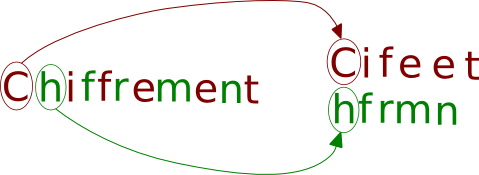
\includegraphics[scale=0.4]{images/Transposition.png}
  \end{center}
  \caption{Le chiffre \emph{Rail Fence}, sur deux lignes}
  \label{fig:Transposition}
\end{figure}

La plupart des chiffres de transposition utilisent des tableaux pour
chiffrer, il suffit alors d'écrire le message initial dans un tableau
d'une taille donnée, et de faire quelques opérations sur ce tableau
afin de «~mélanger~» les lettres. On peut facilement représenter cela
à l'aide des matrices : utilisons une matrice de 5
colonnes, dans laquelle nous écrivons «~chiffrement par transposition
». Un problème se pose alors pour la dernière ligne, elle n'est pas
complète ; deux choix s'offrent alors à nous : 
\begin{itemize}
  \item Laisser ces cases vides
  \item Utiliser des «~caractères nuls~», caractères aléatoires qui ne
    servent qu'à compléter la matrice et éventuellement à perturber la
    cryptanalyse du message chiffré.
\end{itemize}
Pour cet exemple, nous allons choisir la seconde méthode, et ajouter
les caractères G, O, K et Z à la fin de la matrice (figure
\ref{fig:TranspositionMatriceNul}).
\begin{figure}[h]
  \begin{center}
  $
  \left(
    \begin{array}{ccccc}
      C & H & I & F & F \\
      R & E & M & E & N \\
      T & P & A & R & T \\
      R & A & S & P & O \\
      S & I & T & I & O \\
      N & G & O & K & Z 
    \end{array}
  \right)
  $
  \end{center}
  \caption{Le message écrit sous forme de matrice, avec l'ajout de
    caractères nuls}
  \label{fig:TranspositionMatriceNul}
\end{figure}

Ensuite, nous allons changer l'ordre des colonnes en attribuant un
nombre à chacune des colonnes, et en les replaçant dans l'ordre des
nombres attribués. Le message chiffré se lira alors verticalement.
Nous pouvons éventuellement réitérer cette opération, c'est ce qu'on
appelle la \emph{double transposition} (et ce qui rends la cryptanalyse plus
compliquée).

Les numéros attribués aux colonnes constitueront la clé ; pour
faciliter la mémorisation de celle ci, nous pouvons utiliser un mot,
ou chaque lettre sera numérotée selon l'ordre alphabétique. Quand une
lettre apparait plus d'une fois, la lettre la plus à gauche aura
l'indice le plus faible, la plus à droite l'indice le plus fort.

Utilisons ici la clé «~Pomme~», ce qui donne «~54231~» en chiffres,
nous réarrangons donc les colonnes selon cet ordre (la dernière
colonne sera la première, la troisème la seconde, ...)

\begin{figure}[h]
  \begin{center}
  $
  \left(
    \begin{array}{ccccc}
      F & I & F & H & C \\ 
      N & M & E & E & R \\
      T & A & R & P & T \\
      O & S & O & A & R \\
      O & T & I & I & S \\
      Z & O & K & G & N
    \end{array}
  \right)
  $
  \end{center}
  \caption{La matrice réarrangée, selon la clé «~Pomme~»}
  \label{fig:TranspositionMatriceCode}
\end{figure}

Ainsi, le message codé sera «~FNTOOZIMASTOFEROIKHEPAIGCRTRSN~», et on
pourra facilement le déchiffrer en le réécrivant verticalement dans
une matrice possédant le même nombre de colonnes que la clé (5 ici),
en numérotant les colonnes de droite à gauche et en les remettant dans
l'ordre de la clé.

Nous avons utilisé ici un chiffre de transposition par colonnes, mais
il y a de nombreuses possibilitées : par lignes, en diagonales, en
spirale, ...
